\documentclass[titlepage, 12pt]{book}
\usepackage[spanish]{babel}

\pagestyle{plain}
\title{Falluto2.0 Un Model Checker para la verificaci\'on autom\'atica de sistemas tolerantes a fallas.}
\author{Raul Monti}
\date{Diciembre 2012}

\usepackage{graphicx} %para poner imágenes
\usepackage{float} % para establecer posición de imágenes
\usepackage{amsmath} % para etiquetar flechas
\usepackage{tabularx}

\begin{document}

%TODO cambiar las palabras entre []
%TODO rellenar los '...'
\maketitle

\newpage
ACA VA EL RESUMEN
\newpage
ABSTRACT
\newpage
AGRADECIMIENTOS

\newpage
\tableofcontents

\newpage



\chapter{Introducci\'on}
\label{introduccion}

Es f\'acil notar la amplia dependibilidad que las personas hemos formado alrededor de dispositivos computacionales. A medida que crece la confianza hacia estos dispositivos para la realizaci\'on de diferentes tareas, crece tambi\'en el peligro que puede acarrear la ocurrencia de una falla en los mismos. En algunos casos, las actividades a las que son dedicados estos sistemas son actividades de bajo riesgo, como por ejemplo en un reloj de pulsera o un reproductor de m\'usica, y el incorrecto funcionamiento de los mismos no ocasiona da\~nos mayores. En otros casos las actividades realizadas son de car\'acter cr\'itico, como es por ejemplo en el caso de controladores de vuelo, o controladores de compuertas de contenci\'on fluvial. Es en estos \'ultimos donde el incorrecto funcionamiento del sistema puede provocar grandes [perdidas] monetarias y hasta llegar a ocasionar la [perdida] de vidas humanas.\\

Podemos considerar a la falla en una componente de hardware o software como una desviaci\'on de su funci\'on esperada. Las fallas pueden surgir durante todas las etapas de evoluci\'on del sistema computacional - especificaci\'on, dise\~no, desarrollo, elaboraci\'on, ensamblado, instalaci\'on- y durante toda su vida operacional\cite{faultInjection} (debido a eventos externos). Este comportamiento fuera de lo normal puede llevar a un falla funcional del sistema, provocando que se comporte de manera incorrecta, o simplemente deje de funcionar.\\
Es importante entonces, para lograr una mayor confiabilidad del software (confiabilidad de que se comporte como su especific\'on plantea) tomar acci\'on sobre la ocurrencia de estas fallas. Existen diferentes enfoques para tratar con fallas. Uno de ellos es elaborar sistemas tolerantes a fallas. A diferencia de otros enfoques en los que se busca eliminar o disminuir la ocurrencia de fallas, en estos sistemas se busca disminuir los efectos de las fallas y en el mejor de los casos recuperarse de estos y evitar que acarreen en fallas funcionales del sistema.\\

Queda claro entonces que un sistema tolerante a fallas provee grandes ventajas en comparaci\'on a uno que no contempla la ocurrencia de las mismas. Al igual que con el resto de los sistemas computacionales, es conveniente comprobar la correctitud de los sistemas tolerantes a fallas.
El dise\~no de algoritmos de tiempo real distribuidos tolerantes a fallas es notoriamente dificil y \emph{propenso a errores}: la combianaci\'on de la ocurrencia de fallas, conviviendo con eventos concurrentes, y las variaciones en las duraciones de tiempos reales llevan a una explosi\'on de estados que [genera una gran demanda] a la capacidad intelectual del dise\~nador humano\cite{SteinerRushby}.\\
En un mundo idealizado, los algoritmos son derivados por un proceso sistem\'atico conducido por argumentos formales que aseguran su correcci\'on respecto a la especificaci\'on original. En cambio, en la realidad contempor\'anea, los dise\~nadores suelen tener un argumento informal en mente y desarrollan el algoritmo final y sus par\'ametros explorando variaciones locales contra este argumento y contra escenarios que resalten casos dif\'iciles o problem\'aticos. La exploraci\'on contra escenarios puede ser parcialmente automatizada usando un simulador y prototipos \'agiles y esta automatizaci\'on puede llegar a incrementar el n\'umero de escenarios que ser\'an examinados y la confiabilidad de la examinaci\'on.\\ La examinaci\'on autim\'atica de escenarios puede ser llevada a un nivel a\'un m\'as avanzado usando \emph{Model Checking} \cite{SteinerRushby}.\\

En ciencias de la computaci\'on \emph{Model Checking} refiere al siguiente problema: dada una estructura formal del modelo de un sistema, y dada una propiedad escrita en alguna l\'ogica espec\'ifica, verificar de manera autom\'atica y exhaustiva si la el sistema satisface la propiedad. El sistema normalmente representa a un componente de hardware o software, y la f\'ormula a cumplirse representa una propiedad de \emph{safety} o \emph{liveness} que se desea verificar que el sistema cumpla, y de esta manera incrementar la confiabilidad sobre el mismo.
El reducido nivel de interacci\'on con el usuario de este m\'etodo es visto como un ventaja para la aplicaci\'on en la industria, ya que incrementa las posibilidad des ser usad por individuos no expertos\cite{RuysBrinksma}.\\
%TODO quiz\'as quitar esto y ponerlo en la seccion que sigue 
Sin embargo es preciso modelar el sistema y definir las propiedades, lidiando mientras tanto con el principal problema del Model Checking: \emph{la explosi\'on de estados} debido al incremento exponencial de los mismos a ra\'iz de la introducci\'on de variables en la especificaci\'on del sistema.\\

Es objetivo de este trabajo elaborar una herramienta que logre contribuir a disminuir los problemas al momento de verificar sistemas tolerantes a fallas. Por un lado se intenta evitar la introducci\'on de errores en el modelado del sistema en el que conviven fallas con procesos concurrentes. Por otro lado se busca evitar la introducci\'on excesiva de nuevas variables al representar el comportamiento de las fallas, evitando as\'i la nociva explosi\'on de estados al momento de la verificaci\'on.

Para ello presentamos la herramienta de model checking \emph{Falluto2.0}, orientada a la verificaci\'on de sistemas tolerantes a fallas. Esta herramienta presenta una capa de abstracci\'on sobre NuSMV\cite{NuSMV}, un model checker basado en diagramas de decisi\'on binaria. Falluto2.0 presenta un lenguaje de car\'acter declarativo para la introducci\'on de fallas en el modelado del sistema, generando un marco de seguridad contra la introducci\'on de errors evitando que el usuario deba explicitar el funcionamiento de la falla dentro del modelo.\\Este trabajo se presenta como extensi\'on tanto del trabajo realizado por Edgardo Hammes\cite{Falluto1} como del realizado por Nicol\'as Bordenabe\cite{Offbeat}.
%TODO seguir hablando del trabajo y poner la distribucion de los temas en el trabajo.





%%%%%%%%%%%%%%%%%%%%%%%%%%%%%%%%%%%%%%%%%%%%%%%%%%%%%%%%%%%%%%%%%%%%%%%%%%%%%%%%%%%%%%%%%%%%%%%%%%%%%%%%%%%%%%%%%%%%%%%%%%%%%%%%%%%%%%%%%%%%%%%%%%%%%%%%%%%%%%%%%%




\chapter{Tolerancia a fallas}

Mejorar la confiabilidad del sistema (el grado de confianza que se puede poner 
de manera justificada sobre el sistema) es usualmente presentado como el 
principal beneficio de la tolerancia a fallas. <Normalmente la confiabilidad es 
definida estad\'isticamente, indicando la probabilidad de que el sistema sea 
funcional y provea el servicio esperado en un alg\'un momento espec\'ifico >?
\cite{Felix}.




%..................................................................................................................................................................



\section{Fallas}
Intuitivamente, y dentro del contexto que nos competen, podemos definir a una falla como una desviaci\'on de su funci\'on esperada en una componente de hardware o software. Estas fallas pueden ocurrir en cualquier etapa de la evoluci\'on del sistema computacional en cuesti\'on -especificaci\'on, dise\~no, desarrollo, elaboraci\'on, ensamblado, e instalaci\'on- y durante toda su vida operacional\cite{FaultInject}.\\

Una definici\'on ligeramente m\'as formal nos sugiere definir el termino 'falla' basado en la observaci\'on de que los sistemas cambian su estado como resultado de dos clases de eventos muy similares: operaciones normales de sistema y ocurrencia de fallas. Por lo tanto, un falla puede ser modelada como una no deseada (pero sin embargo posible) transici\'on de estado en un proceso\cite{Felix}.



%..................................................................................................................................................................



\section{Sistemas tolerantes a fallas}
Existen sistemas dise\~nados para ser tolerantes a fallas: ellos o bien exhiben un bien definido comportamiento ante fallas cuando estas ocurren, o bien enmascaran la falla de la componente al usuario, es decir contin\'uan proveyendo su servicio est\'andar especificado a pesar de la ocurrencia de las fallas en la componente\cite{Cristian}.
Podemos entonces decir de manera vaga que la tolerancia a fallas es la habilidad que posee un sistema de comportarse de una manera bien definida ante la ocurrencia de una falla. En el momento de dise\~nar la tolerancia a fallas, un primer prerrequisito es especificar la clase de falla que ser\'a tolerada. Tradicionalmente esto se lograba usando como base alguno de los modelos de fallas est\'andares (crash, fail-stop, etc...), sin embargo puede hacerse de manera mas concisa especificando clases de fallas. El siguiente paso es enriquecer el sistema bajo consideraci\'on con componentes o conceptos que provean protecci\'on contra las fallas de una clase espec\'ifica\cite{FaultInject}.\\

En este trabajo podremos distinguir dos clases de fallas en particular. Un primer grupo de fallas es de tipo \textbf{permanente}: \'estas com\'unmente representan fallas reales causadas por problemas irreversibles en la componente. Una vez que una falla permanente ocurre, permanece activa y afectando al sistema durante el resto de su ejecuci\'on. Por otro lado, un segundo grupo de fallas se caracteriza por ser de duraci\'on instant\'anea. Afectan el estado del sistema en los puntos particulares de se ejecuci\'on en los cuales estas fallas ocurren, sin tener efectos permanentes sobre el mismo. Las mismas pueden repetirse indefinidamente durante la ejecuci\'on del sistema, permaneciendo activas solo en el momento en que afectan al sistema. Diremos que estas fallas son de clase \textbf{transient}.



%..................................................................................................................................................................



\section{Conclusi\'on}
En este trabajo entonces no realizaremos mayor diferencia formal entre transiciones buenas del sistema y transiciones debido a fallas, ambas ser\'an consideradas como transiciones posibles del sistema que podr\'an afectar o no el estado del mismo.\\

Distinguiremos adem\'as como dijimos dos clases de falla, las de tipo \textit{Permanente} y las de tipo \textit{Transient}.\\

Por \'ultimo, nos ocuparemos del modelado del sistema en general y nos centraremos en la inyecci\'on de las fallas en el mismo. No nos detendremos sin embargo en temas espec\'ificos al dise\~no de la tolerancia a las fallas.






%%%%%%%%%%%%%%%%%%%%%%%%%%%%%%%%%%%%%%%%%%%%%%%%%%%%%%%%%%%%%%%%%%%%%%%%%%%%%%%%%%%%%%%%%%%%%%%%%%%%%%%%%%%%%%%%%%%%%%%%%%%%%%%%%%%%%%%%%%%%%%%%%%%%%%%%%%%%%%%%%%





\chapter{Model Checking}

En el dise\~no de software y hardware de sistemas complejos, se consume mas tiempo y esfuerzo en verificaci\'on que en construcci\'on. Se entiende que la aplicaci\'on de t\'ecnicas reduce y aligera los esfuerzos en verificaci\'on a la vez que acrecientan su cobertura. Los m\'etodos formales ofrecen un gran potencial para obtener una integraci\'on temprana de la verificaci\'on en el proceso de dise\~no, para proveer de t\'ecnicas de verificaci\'on mas afectivas y reducir el tiempo invertido en aplicarlas\cite{prinMC}.\\

El \textbf{Model Checking} es un m\'etodo formal para la verificaci\'on exhaustiva de sistemas finitos. Logra esta verificaci\'on explorando todos los estados posibles del sistema con la intenci\'on de verificar la veracidad de una propiedad sobre el mismo.\\

En este cap\'itulo comenzaremos revisando algunos conceptos b\'asicos para entender el funcionamiento de los \textit{model checkers} (programas utilizados para la verificaci\'on mediante \textit{model checking}, y concluiremos presentando el proceso de \textit{model checking} junto con algunas caracter\'isticas de este m\'etodo.





%..................................................................................................................................................................




\section{Sistemas de transici\'on}
%TODO introducir sistemas de transicion

\subsection{Labelled transition systems - LTS}
Llamamos sistema de transiciones etiquetadas a un concepto de maquina abstracta usada en parte para el modelado de sistemas computacionales concurrentes. Este sistema de representaci\'on est\'a compuesto por un conjunto de estados, un conjunto de etiquetas o nombres, y una relaci\'on ternaria explicando las transiciones etiquetadas desde un estado hacia otro del sistema.\\
Formalmente podemos decir que un LTS es una tres-upla $M = (S,S_{0},L,R)$ donde:
\begin{itemize}
\item $S$ es un conjunto (de estados)
\item $S_0 \subseteq S$ es un conjunto de estados denominados iniciales
\item $L$ es un conjunto de etiquetas (nombres de transiciones)
\item $R \subseteq S \times L \times S$ es una relaci\'on ternaria (de transiciones etiquetadas)
\end{itemize}
Notemos entonces que si s1 y s2 son elementos en S, l es un nombre en L, y (s1,l,s2) pertenece a R, entonces estamos indicando que existe una transici\'on con nombre l desde el estado s1 al estado s2.\\
As\'i podemos modelar sistemas computacionales tomando cada elemento en S como un estado particular del sistema y definiendo relaciones etiquetadas entre los mismos para representar el comportamiento del sistema.\\

En particular nos interesa para este trabajo la capacidad que nos otorga este formalismo para representar sincronizaci\'on entre acciones de distintas componentes del sistema. En el ejemplo de la figura \ref{figura1} encontramos dos componentes, un productor y un consumidor, ambas con su representaci\'on LTS. Podemos a partir de ellas definir un sistema concurrente sincronizado en el cual las transiciones de igual nombre en cada componente deben ser ejecutadas de manera sincronizada, mientras que las transiciones propias de cada componente pueden ejecutarse independientemente. Vemos el sistema resultante en la figura \ref{figura2}. En ella la transici\'on punteada y etiquetada con 'Listo' representa la acci\'on sincronizada entre el productor y el consumidor. A su vez podemos ver en el estado punteado un caso de [interliving] entre los procesos sincronizados. All\'i podemos elegir entre darle paso a la acci\'on 'Producir' del productor, o dejar que el consumidor realice la acci\'on 'Consumir'. 


\begin{figure}[H] %Al incluir el paquete float, [H] obliga a posicionar la imagen justo en este lugar por mas que a latex no le guste.
  \centering
    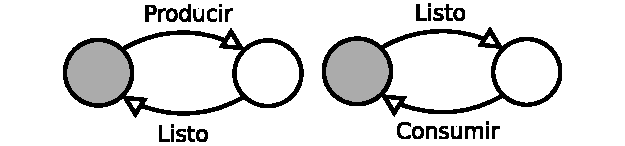
\includegraphics{Imagenes/prodYcons.pdf}
  \caption{El productor (izquierda) y el consumidor (derecha).}
  \label{figura1}
\end{figure}
~\\\\

\begin{figure}[H] %Al incluir el paquete float, [H] obliga a posicionar la imagen justo en este lugar por mas que a latex no le guste.
  \centering
    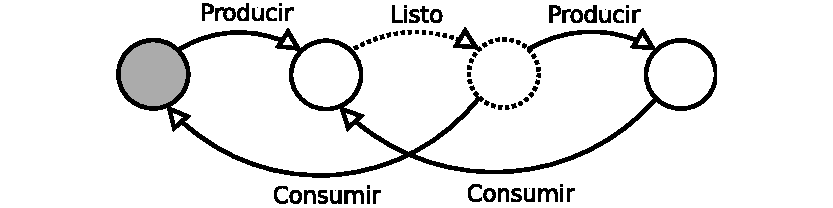
\includegraphics{Imagenes/prodYconsSincro.pdf}
  \caption{productor y consumidor de la figura \ref{figura1} sincronizados.}
  \label{figura2}
\end{figure}
~\\\\

\subsection{Estructuras de Kripke}
En model checking usamos un tipo de grafos de transición de estados llamados \textit{Structuras de Kripke} para intuitivamente captar el comportamiento del sistema a modelar. Una \textit{estructura de Kripke} consiste en un conjunto de estados, un conjunto de transiciones entre esos estados, y una función que etiqueta cada estado con un conjunto de propiedades que son verdaderas en este estado. Los caminos en estas estructuras modelan la ejecución del sistema\cite{Clarke}. Estas estructuras son lo suficientemente expresivas como para captar aspectos de lógicas temporales tales como (LTL y CTL) que interesan a la verificación de sistemas vía model checking.\\

Formalmente podemos definir una estructura de Kripke como sigue\cite{Clarke}:\\

Sea AP un conjunto de proposiciones at\'omicas. Una estructura de Kripke M sobre AP es una cuatro-upla (S,$S_0$,R,L) tal que:
\begin{enumerate}
\item S es un conjunto finito de estados.
\item $S_0$ $\subseteq$ S es un conjunto de estados inciales.
\item R $\subseteq$ S x S es una relaci\'on de transici\'on que debe ser total, es decir, para cada estado s $\in$ S hay un estado s' $\in$ S tal que R(s,s').
\item L : S x $2^{AP}$ es una funci\'on que etiqueta cada estado con el conjunto de proposiciones atómicas verdaderas en ese estado.
\end{enumerate}
Una ejecuci\'on del sistema desde un estado s es representado en la estructura M como una secuencia infinita $\pi = s_0s_1s_2...$ tal que $s_0$ = s y $R(s_i,s_{i+1})$ vale para todo i $\geq$ 0.\\

Notemos que podemos traducir la representación LTS de un sistema a una representaci\'on en Estructuras de Kripke equivalente de la siguiente manera. Sea $M_1 = (S_1, S_{1_0} R_1, L_1)$ un sistema descripto en LTS, entonces construimos su descripci\'on $M_2 = (S_2,S_{2_0},R_2,L_2)$ en t\'erminos de estructuras de Kripke sobre AP de la siguiente manera:
\begin{itemize}
\item $ AP = \{action = e ~|~ e \in L_1 \cup \{null\}\} $
\item $ S_2 = S_1 \times (L_1 \cup \{null\}) $
\item $S_{2_0} = S_{1_0} \times \{null\}$
\item $R_2 = \{(s,a) \rightarrow (s',b) ~|~ s\overset{b}{\rightarrow}s' \in R_1, a \in L \cup \{null\}\}$
\item $L_2(s,a) = (action = a), ~\forall~(s,a) \in S_2$
\end{itemize}
Lo que hicimos fue entonces construir por cada estado $s_i$ y etiqueta $e$ en el LTS un estado en la estructura de Kripke que represente llegar al estado $s_i$ usando la etiqueta $e$. Dado que en el inicio de las ejecuciones no realizamos acci\'on alguna para llegar al estado inicial, es que hemos adem\'as definido para cada estado $s \in S_{1_0}$ un estado $(s,null)$ que lo represente en $S_2$. La funci\'on de relaci\'on se forma de manera intuitiva. El etiquetado indica qu\'e acci\'on se llev\'o a cabo para llegar a cada estado. Esto \'ultimo, junto con el nombre del estado, dejan en claro la transici\'on llevada a cabo en la ejecuci\'on del sistema definido en el LTS original. Vemos un ejemplo de traducci\'on LTS-Kripke en la figura \ref{ltsakripke}. Notemos que el sistema traducido puede ser depurado quitando estados no alcanzables como se muestra en la tercera figura de \ref{ltsakripke}.

\begin{figure}[H]
  \centering
    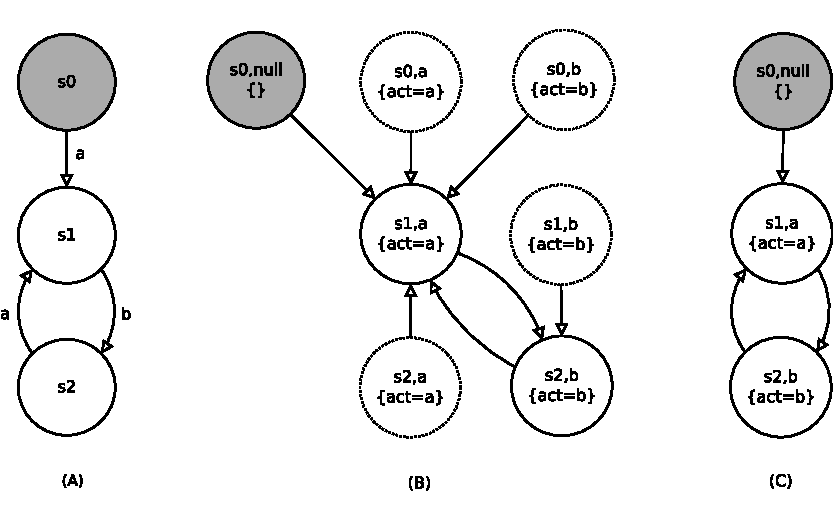
\includegraphics{Imagenes/ltsakripke.pdf}
  \caption{Ejemplo de traducci\'on de un sistema LTS a estructuras de Kripke. (A) El sistema en LTS; (B) El sistema en estructuras de Kripke; (C) El sistema en estructuras de Kripke depurado}
  \label{ltsakripke}
\end{figure}
~\\\\



%..................................................................................................................................................................



\section{De estructuras de Kripke a f\'ormulas \text{l\'ogicas}}
Si bien las estructuras de Kripke nos sirven para captar intuitivamente el comportamiento de los sistemas a modelar, los model checkers trabajan sobre el modelado del sistema en base a la l\'ogica de primer orden. A continuaci\'on veremos como lograr la interpretaci\'on de estructuras de Kripke usando f\'ormulas l\'ogicas de primer orden. En lo que a nosotros concierne, la l\'ogica de primer orden estar\'a comprendida por los conectivos l\'ogicos usuales - $\neg,\wedge,\vee,\rightarrow,etc...$ -, y haremos uso tambi\'en de los cuantificadores $\forall$ y $\exists$.\\

Supongamos que queremos modelar un sistema $P$, y tomemos todas sus variables de sistema $V = {v_0,v_1,...,v_n}$. Consideremos para el caso que todas estas variables toman valores de un domino finito $D$. Tenemos que una valuaci\'on de $V$ es una funci\'on total sobre el dominio, la cual asigna a cada variable en $V$ un valor en $D$. Notemos que dado que los valores de las variables del sistema son las que definen el estado del mismo en su totalidad, cada valuci\'on estar\'ia definiendo el estado del sistema. Por lo tanto en t\'erminos de estructuras de Kripke tenemos que si $M = (S,S_0,R,L)$ sobre $AP$ modela un sistema con variables en V entonces:
\begin{itemize}
\item $\textit{Usualmente } AP = \{v=d~|~ v \in V, d \in D\}.$
\item \textit{Cada estado s $\in$ S es una valuaci\'on sobre V.}
\item \textit{R explica la relaci\'on entre estas valuaciones, vale decir explica la transici\'on entre los cambios de valores en las variables del sistema.}
\item \textit{L(s) es el subconjunto de proposiciones en AP que son validas dada la valuaci\'on del estado s.}
\end{itemize}
Dada un estado en la estructura de Kripke, es decir una valuaci\'on $s:V\rightarrow D$, podemos escribir una f\'ormula sobre las variables en V tal que sea v\'alida solo para esta valuaci\'on\cite{Clarke}. La f\'ormula ser\'ia: $$(v_0 = s(v_0)) \& (v_1 = s(v_1)) \& ... \& (v_n = s(v_n))$$
Dado que en general una f\'ormula puede ser satisfecha por diferentes valuaciones, podemos a partir de ella definir el conjunto de estados que la satisfacen. Asi por ejemplo podemos definir una f\'ormula cuyos estados que la satisfacen sean solo los estados iniciales del sistema ($S_0$ en la estructura de Kripke que lo modela).\\

Adem\'as de definir los estados, necesitamos poder especificar tambi\'en transiciones como f\'ormulas interpretadas de primer orden. Para ello debemos lograr a partir de una f\'ormula representar la relaci\'on entre una valuaci\'on actual y la siguiente (estado actual y estado sucesor). Necesitaremos entonces otro conjunto de variables $V'$ el cual representen las variables en estado sucesor. De esta forma, dada la f\'ormula de transici\'on $F_r$ sobre el conjunto de variables $V \cup V'$ diremos que $s'$ es estado sucesor de $s$, es decir que $(s,s')\in R$, si y solo si $F_r$ es v\'alida al valuar todas sus variables en $V$ seg\'un $s$ y todas sus variables en $V'$ seg\'un $s'$.\\

Por \'ultimo, las proposiciones en AP nos permiten definir propiedades sobre los estados. Recordemos que las proposiciones at\'omicas en AP son de la forma $v=d$ con $v \in V$ y $d \in D$. Entonces tenemos que una proposici\'on $v=d$ es v\'alida en el estado $s$ si y solo si $d = s(v)$. En tal caso tenemos que $v=d \in L(s)$.




%..................................................................................................................................................................




\section{Representaci\'on de f\'ormulas l\'ogicas en BDD}






%..................................................................................................................................................................





\section{L\'ogicas temporales}
Las l\'ogicas temporales son sistemas de reglas y s\'imbolos que nos permiten describir y razonar sobre proposiciones en t\'erminos del tiempo. En el caso del model checking, son de gran utilidad para la especificaci\'on de las propiedades a verificar sobre el modelo del sistema. A continuaci\'on presentaremos dos l\'ogicas temporales de inter\'es para este trabajo. Ambas l\'ogicas difieren en expresividad, por lo que hacer uso de las dos nos permite una mayor versatilidad al momento de especificar las propiedades deseadas.\\

\subsection{LTL}
La \textbf{L\'ogica de Tiempo Lineal (LTL)} nos permite razonar sobre ejecuciones lineales a trav\'es del tiempo. En cada instante de tiempo solo existe una \'unica ejecuci\'on real a realizarse. Comúnmente esta ejecuci\'on de la que hablamos comienza en este momento y se extiende al infinito. El tiempo es discreto y podemos realizar un paralelismo entre el salto de un momento al otro y cada paso en la ejecuci\'on del sistema que se analice. As\'i, cada momento representa una configuraci\'on en el estado del sistema y cada salto en el tiempo representa una transici\'on desde un estado del sistema a uno nuevo. Estas l\'ogicas est\'an compuestas por un conjunto finito de proposiciones at\'omicas AP, los conectivos booleanos $\neg$, $\wedge$, $\vee$, $\rightarrow$, $\leftrightarrow$ y los conectivos temporales G, F, X, U, R. Estos \'ultimos conectivos se corresponden con las palabras en idioma ingl\'es \textbf{G}lobally, \textbf{F}inally, Ne\textbf{X}t, \textbf{U}ntil y \textbf{R}elease.\\ A continuaci\'on damos una descripci\'on intuitiva del significado de cada conectivo:
\begin{itemize}
\item G $\phi$ expresa que en todo momento vale $\phi$.
\item F $\phi$ expresa que $\phi$ se cumple en elg\'un momento.
\item X $\phi$ expresa que $\phi$ se cumple en el momento inmediatamente posterior al actual.
\item $\phi$ U $\psi$ expresa que $\psi$ vale en alg\'un momento, y para todo momento anterior a aquel $\phi$ vale.
\item $\phi$ R $\psi$ expresa que o bien $\phi$ no vale nunca y $\psi$ vale siempre, o bien $\psi$ vale en cada momento hasta que $\phi$ valga.
\end{itemize}
Usando LTL podemos expresar propiedades de \textit{safety} y \textit{liveness} de nuestro sistema de manera sencilla. Por ejemplo para expresar \textit{En alg\'un momento algo bueno suceder\'a} usamos  \textbf{F} 'algoBueno', o para expresar \textit{En ning\'un momento algo malo sucede} usar\'iamos \textbf{G} $\neg$ 'algoMalo'.\\

Es común interpretar las f\'ormulas LTL sobre estructuras de Kripke. Una f\'ormula LTL puede ser satisfecha por una serie infinita de valuaciones sobre AP. Podemos ver a esta serie infinita como una palabra sobre una ejecuci\'on sobre una estructura de Kripke. De este modo si queremos saber si la formula $\phi$ se satisface en un sistema representado por la estructura de Kripke M, basta con ver que el lenguaje de M (todas las palabras posibles en M) satisfagan $\phi$. Definimos la sem\'antica de formulas LTL como sigue:\\

Sea la palabra $\omega$ = $s_1s_2s_3...$ de valuaciones en AP. Definimos la relaci\'on de satisfactibilidad $\models$ de una formula LTL con respecto a la palabra $\omega$ a partir de las siguientes reglas:
\begin{itemize}
\item $\omega \models p $ si $ p \in \omega[0]$
\item $\omega \models \neg p $ si no $\omega \models p$
\item $\omega \models \phi \vee \psi$ si $\omega \models \phi$ or $\omega \models \psi$
\item $\omega \models$ X $\phi$ si $\omega$[1...] $\models \phi$
\item $\omega \models \phi U \psi$ si existe $i \geq 0$ tal que  $\omega[i...] \models \psi$ y para todo $0 \leq k < i$, $\omega[k...] \models \phi$ 
\end{itemize}
Notar que los dem\'as conectivos son derivados de aquellos para los que hemos definido las reglas de satisfactibilidad. \\

Muchas veces es de inter\'es en model checking definir propiedades bajo \textbf{condiciones de equidad}, tambi\'en llamadas \textit{condiciones de \textbf{fairness}}. Por ejemplo en el contexto del modelado de un planificador de tareas podemos requerir que el mismo atienda equitativamente a los diferentes procesos. LTL a diferencia de CTL nos da la posibilidad de definir estas equidades:
\begin{enumerate}
\item Equidad incondicional: G F p (siempre finalmente se cumple p, o a menudo se cumple p)
\item Equidad fuerte: G F q $\rightarrow$ G F p (si a menudo vale q entonces a menudo vale p)
\item Equidad d\'ebil: F G q $\rightarrow$ G F p (si finalmente siempre vale q, entonces a menudo vale p)
\end{enumerate}


\subsection{CTL}
A diferencia de LTL, en la \textbf{L\'ogica de \'Arbol Computacional (CTL)} no existe en cada momento un \'unico camino a seguir. CTL es una l\'ogica de tiempo ramificado, en cada momento consideramos todos los posibles saltos hacia un estado posterior, y por lo tanto consideramos diferentes ejecuciones como posibles a realizarse en el futuro. Adem\'as de los conectivos l\'ogicos y temporales introducidos en LTL, CTL implementa el uso de los cuantificadores \textbf{A} (para todo camino) y \textbf{E} (existe un camino). A su vez establece la regla de estar obligado a usar estos cuantificadores delante de cada conectivo temporal, definiendo as\'i f\'ormulas sobre estados y no sobre caminos como lo hacen la l\'ogica LTL. CTL, a diferencia de LTL, nos permite hablar sobre la existencia de al menos un camino. Así es que podemos especificar propiedades como  \textit{E X p} y \textit{AG EF p}, las cuales no pueden ser especificadas en LTL ya que en ella no podemos hablar de la existencia de al menos un camino en el futuro en el cual se cumple 'p'.

Los conectivos ${\neg,\wedge,AX,AU,EU}$ comprenden un conjunto completo de conectivos para la l\'ogica CTL dado que los dem\'as pueden ser derivados a partir de ellos. Podemos decir que el siguiente es el significado intuitivo de estos conectivos:
\begin{itemize}
\item $\neg$ es la negaci\'on booleana usual.
\item $\wedge$ es la conjunci\'on booleana usual.
\item $AX~q$ se cumple en un estado $s$ si para cualquier ejecuci\'on, $q$ vale en el estado que sucede a $s$.
\item $EX~q$ se cumple en un estado $s$ si existe al menos una ejecuci\'on donde $q$ vale en el estado que sucede a $s$.
\item $E[p~U~q]$ se cumple en un estado $s$ si existe al menos una ejecuci\'on $s_1s_2...s_n...$ con $s_1 = s$ donde $q$ vale en $s_n$ y $p$ vale para todo estado en $s_1...s_{n-1}$.
\end{itemize}

A continuaci\'on, utilizando estructuras de Kripke, definimos la sem\'antica formal de CTL por inducci\'on estructural sobre una f\'ormula $\phi$. Sea la estructura de Kripke $M =(S,S_0,R,L)$ sobre AP, sea $\phi$ una f\'ormula CTL bien formada sobre AP, y sean s $\in$ S y p $\in$ AP.\\

\begin{tabularx}{\textwidth}{@{\textbullet}lcX}
$~M,s \models p$ & $\leftrightarrow$ & $p \in L(s)$\\
$~M,s \models \neg\phi $ & $\leftrightarrow$ & $ \text{no } M,s \models \phi$\\
$~M,s \models \phi_0 \wedge \phi_1 $ & $\leftrightarrow$ & $ M,s \models \phi_0 \text{ y } M,s \models \phi_1$\\
$~M,s \models AX\phi $ & $\leftrightarrow$ & $ \forall (s,s') \in R,~ M,s' \models \phi$\\
$~M,s \models EX\phi $ & $\leftrightarrow$ & $ \exists (s,s') \in R,~M \text{ tal que } s' \models \phi$\\
$~M,s \models E(\phi_0 U \phi_1) $ & $\leftrightarrow$ & $\exists \text{ una ejecuci\'on } s_1s_2s_3...s_n... \text{ definida por } R \text{ tal que }\linebreak  s_0 = s, M,s_n \models \phi_1, \forall 0<i<n~ M, s_i \models \phi_0$\\
\end{tabularx}




%..................................................................................................................................................................




\section{Caracter\'isticas del Model Checking}
Existen diferentes m\'etodos para la verificaci\'on de sistemas complejos, entre ellos podemos destacar como principales la simulaci\'on, el testing, la verificaci\'on deductiva, y el model checking\cite{Clarke}. Tanto la simulaci\'on como el testing comprenden realizar experimentos antes de desplegar el sistema en el campo. Mientras que en el caso de la \textit{simulaci\'on} se trabaja sobre una abstracci\'on o modelo del sistema, en el \textit{testing} se trabaja sobre el [producto real]. En cuanto a costo-eficiencia, estos m\'etodos pueden ser ventajosos para detectar gran cantidad de errores. Sin embargo, revisar todas las posibles interacciones y potenciales errores usando simulaci\'on y testing es raramente posible.\\
El t\'ermino \textit{verificaci\'on deductiva} normalmente refiere al uso de axiomas y reglas para probar la correctitud del sistema. Este m\'etodo si bien posee la ventaja de poder probar correctitud sobre sistemas de estados infinitos no es muy utilizado fuera de casos cr\'iticos. Esto se debe a que requiere de gran cantidad de tiempo y de la conducci\'on por parte de expertos en el campo del razonamiento l\'ogico.\\

\textbf{Model checking} es un m\'etodo autom\'atico para la verificaci\'on de propiedades sobres sistemas concurrentes finitos. Trabaja sobre un modelo del sistema y explora exhaustivamente todos sus posibles estados con el fin de verificar si una propiedad especificada sobre el mismo es verdadera o no. Presenta ciertas ventajas sobre los m\'etodos anteriormente mencionados:

\begin{itemize}
\item Detecta errores en etapas tempranas de diseño, evitando tener que replantear todo al encontrar estos errores en etapas posteriores.

\item Gran parte de su proceso es autom\'atico, por lo cual no requiere de personal experto en campos de la matem\'atica para llevar a cabo las tareas de verificaci\'on.

\item Es exhaustivo con respecto al conjunto de estados del sistema.

\item Ofrece clara evidencia del problema en el caso de encontrar que la propiedad deseada sobre el sistema no se cumpla.
\end{itemize}

Sin embargo model checking sufre del problema de explsi\'on de estados. Esto implica que f\'acilmente se llegue a sistemas en los que la cantidad de estados es tan grande que supera los l\'imites de memoria f\'isica del hardware sobre el que corre el programa de model checking. Muchos algoritmos y optimizaciones sobre los model checkers han ayudado a combatir este efecto, pero sin embargo el mismo persiste. Otra soluci\'on a este problema es llevar el modelado a una mayor abstracci\'on con el fin de disminuir la cantidad de estados finales. Al hacer esto debemos tomar en cuenta que la abstracci\'on debe preservar la no satisfactibilidad de las propiedades a verificar, en el caso que esta exista. Como vemos este proceso de abstracci\'on y refinamiento requiere muchas veces de personal experto, y es una de las barreras a superar si se desea lograr que el model checking se convierta enteramente en una herramienta \text{``push-button''}.

Christel Baier y Joost-Pieter Katoen en su libro "Principles of model checking" \cite{baier} identifican las siguientes tareas como pasos para realizar el \textit{proceso de model checking} sobre el dise\~no de un sistema:

\begin{enumerate}
\item Fase de modelado:
\begin{itemize}
\item Modelar el sistema en consideraci\'on usando el lenguaje del model checker que se tenga a mano.
\item Realizar algunas simulaciones sobre el modelo como primera revisi\'on y r\'apida aceptaci\'on del mismo.
\item Describir las propiedades a verificar sobre el modelo usando el lenguaje espec\'ifico para esta tarea.
\end{itemize}
\item Fase de ejecuci\'on:\\\\
Ejecutar el model cheker para verificar la validez de una propiedad sobre el sistema modelado. 
\item Fase de an\'alisis:
\begin{itemize}
\item Si la propiedad result\'o ser v\'alida $\longrightarrow$ en el caso de haber mas propiedades a verificar, proceder con la verificaci\'on de las mismas.
\item Si la pripiedad fu\'e refutada $\longrightarrow$
\begin{enumerate}
\item analizar, a partir de simulaci\'on, el contraejemplo generado.
\item refinar el modelo, diseño o propiedad.
\item repetir todo el proceso.
\end{enumerate}
\item La computadora se qued\'o sin memoria $\longrightarrow$ intentar reducir el modelo y empezar de nuevo.
\end{itemize}
\end{enumerate}




\begin{figure}[H]
  \centering
    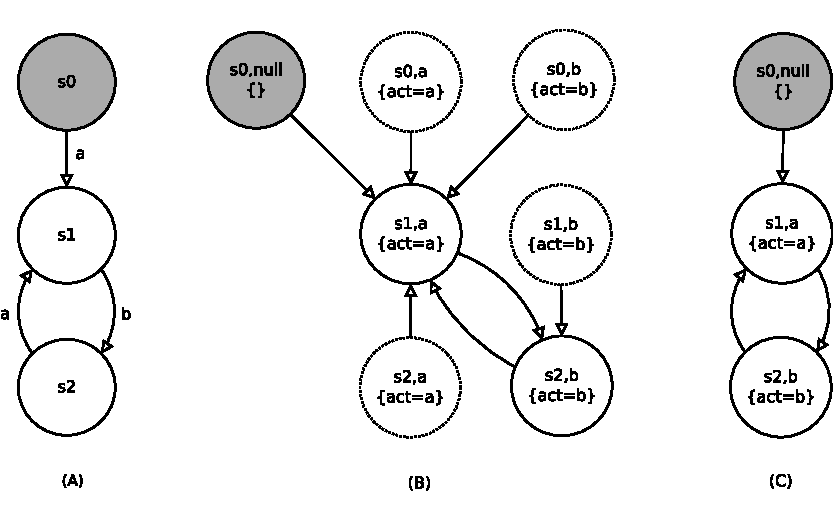
\includegraphics{Imagenes/ltsakripke.pdf}
  \caption{}
  \label{ltsakripke}
\end{figure}
~\\\\








\chapter{Casos de estudio}
			\section{Commit at\'omico}
			\section{Ej\'ercitos bizantinos ?}
			\section{Fil\'osofos comensales ?}
			\section{Falla bizantina ?}
			\section{Elecci\'on de lider ?}
			\section{Protocolos lamport}
			\section{Feedback de contacto de Naza}
			\section{Red satelital ultra secreta?}


\chapter{Conclusi\'on}

\chapter{Ap\'endice A - Manual de Falluto2.0}

\chapter{Ap\'endice B - Sint\'axis formal de Falluto2.0}

\chapter{Ap\'endice C - Ejemplo paradigm\'atico de compilaci\'on.}




\chapter{extra}
	- falencias de falluto??? 
	- fallas por omisi\'on de input.
	- recuperci\'on de fallas por parte del usuario.




%
%\section{\textbf{NuSMV}}
%
%NuSMV\cite{NuSMVBibl} es un model checker simb\'olico originado en la reingenieria, reimplementaci\'on
%y extensi\'on of CMU SMV. Usamos su segunda versi\'on la cual implementa tanto t\'ecnicas
%de \textbf{model checking simb\'olico basado en BDD}, como  t\'ecnicas de model checking
%basadas en \textbf{satisfactibilidad proposisional (SAT)}.
%Cada una de estas t\'ecnicas sulen ser \'utiles para resolver diferentes tipos
%de problemas y por lo tanto pueden considerarse complementarias.\\
%
%El c\'odigo de \emph{NuSMV} se distribuye bajo licencia LGPL-2.1 la cual permite el 
%uso gratuito del software por parte de cualquier persona interesada asi como a 
%contribuir con el desarrollo del mismo. La adopci\'on de esta licencia ha permitido la
%contribuci\'on al proyecto por parte de numerosos \'ambitos cient\'ificos asi como
%industriales.\\
%
%El proyecto de software libre NuSMV apunta a crear una base com\'un para
%el estudio y comparaci\'on de diferentes t\'ecnicas de model checkin simb\'olico.\\
%
%\begin{itemize}
%
%
%\item%
%\textbf{Funcionalidades:}\\
%
%\emph{NUSMV} permite la representaci\'on de sistemas finitos tanto s\'incronos
%como as\'incronos, aunque estos \'ultimos estan deprecados en las versiones superiores
%a la 2.5.0., y al an\'alisis de especificaciones expresadas en CTL (l\'ogica de \'arbol
%computacional) y LTL (l\'ogica temporal lineal).
%
%
%\item%
%\textbf{Arquitectura:}\\
%
%
%\item%
%\textbf{Qualidades de la implementacion:}\\
%
%\emph{NUSMV} esta escrito en ANSI C, y es compatible con POSIX. \emph{NUSMV} usa un avanzado
%paquete de BDD desarollado en Colorado University, y provee una interf\'az general para
%linking con avanzados resolvedores SAT. Esto produce que NUSMV sea muy robusto, portable,
%eficiente, y facil de entender por personas fuera del equipo de desarrollo.\\
%\\
%
%
%\end{itemize}
%
%
%\section{Por qu\'e NuSMV?}
%
%Porque nos da un gran control sobre la eficiencia del checkeo del modelo. Esto se debe
%a que ... (Preguntar bien a Pedro o leer mucho para entender :D)
%
%
%\chapter{Falluto 2.0}
%
%\section{Objetivos}
%\begin{itemize}
%\item%
%Ocultar al usuario las complejidades de tener que definir un sistema usando una herramienta
%con la complejidad de NuSMV.
%\item
%Ocultar las complejidades de definir de manera funcional el comportamiento de fallas,
%presentando una sintaxis declarativa para la especificaci\'on de las mismas.
%\end{itemize}
%
%\section{Implementaci\'on de Falluto 2.0}
%
%Falluto 2.0 esta escrito en Python\cite{Python}. Python es un Lenguaje de programaci\'on interpretado cuya filosof\'ia hace hincapi\'e en una sintaxis limpia que favorezca un c\'odigo legible.
%Se trata de un lenguaje de programaci\'on multiparadigma ya que soporta orientaci\'on a objetos, programaci\'on imperativa y, en menor medida, programaci\'on funcional. Es un lenguaje interpretado, usa tipado din\'amico, es fuertemente tipado y es multiplataforma. Posee una muy completa librer\'ia estadar.
%Es administrado por la Python Software Foundation. Posee una licencia de c\'odigo abierto, denominada Python Software Foundation License,1 que es compatible con la Licencia p\'ublica general de GNU a partir de la versi\'on 2.1.1, e incompatible en ciertas versiones anteriores.
%
%
%\subsubsection{A cerca del valor inicial de actvar\#}
%
%Notar que el valor inicial de esta variable no tiene significado alguno en el
%sistema ya que representa la acci\'{o}n que se realiz\'{o} en el estado anterior para 
%transitar hasta el actual. Dado que el estado actual es el inicial, osea no hubo
%estado anterior, esta variable no representa nada en este momento. Sin embargo
%es importante darle un valor correcto para que no afecte la verificaci\'{o}n de
%propiedades en el sistema smv resultante.\\
%
%\noindent Las opciones para su valor inicial son:\\
%\begin{enumerate}
%
%\item%
%    Un valor incial espec\'{i}fico, que solo se use en este caso.
%\item%
%    Cualquier valor dentro de su dominio.
%\end{enumerate}
%
%
%
%
%
%
%\section{Parsing expresion grammars}
%
%
%Most language syntax theory and practice is based on generative
%systems, such as regular expressions and context-free grammars, in
%which a language is defined formally by a set of rules applied recursively
%to generate strings of the language. A recognition-based
%system, in contrast, defines a language in terms of rules or predicates
%that decide whether or not a given string is in the language.
%The power of generative grammars to express
%ambiguity is crucial to their original purpose of modelling
%natural languages, but this very power makes it unnecessarily difficult
%both to express and to parse machine-oriented languages using
%CFGs. Parsing Expression Grammars (PEGs) provide an alternative,
%recognition-based formal foundation for describing machineoriented
%syntax, which solves the ambiguity problem by not introducing
%ambiguity in the first place. Where CFGs express nondeterministic
%choice between alternatives, PEGs instead use prioritized
%choice. PEGs address frequently felt expressiveness limitations of
%CFGs and REs, simplifying syntax definitions and making it unnecessary
%to separate their lexical and hierarchical components. A
%linear-time parser can be built for any PEG, avoiding both the complexity
%and fickleness of LR parsers and the inefficiency of generalized
%CFG parsing. While PEGs provide a rich set of operators for
%constructing grammars, they are reducible to two minimal recognition
%schemas developed around 1970, TS/TDPL and gTS/GTDPL.\cite{PEG}
%
%
%
%

\newpage % Bibliography goes in new page

\begin{thebibliography}{99}

\bibitem{faultInjection} Fault injection: a method for validating computer-system dependability
Clarke, J.A.; Pradhan, D.K. June.1995 

\bibitem{SteinerRushby} Steiner-etal:DSN04; Wilfried Steiner and John Rushby and Maria Sorea and Holger Pfeifer; Model Checking a Fault-Tolerant Startup Algorithm: From Design Exploration To Exhaustive Fault Simulation; The International Conference on Dependable Systems and Networks, IEEE Computer Society, Florence, Italy, june, 2004

\bibitem{RuysBrinksma} Model Checking: Verification or Debugging?; Theo C. Ruys and Ed Brinksma; Faculty of Computer Science, University of Twente. P.O. Box 217, 7500 AE Enschede, The Netherlands.

\bibitem{NuSMV} NuSMV 2.5 User Manual. Roberto Cavada, Alessandro Cimatti, Charles Arthur Jochim, Gavin Keighren,
Emanuele Olivetti, Marco Pistore, Marco Roveri and Andrei Tchaltsev. http://nusmv.fbk.eu/NuSMV/userman/v25/nusmv.pdf

\bibitem{Falluto1} Falluto: Un model checker para la verificaci\'on de sistemas tolerantes a fallas; Edgardo E. Hames; Facultad de Matem\'atica, Astronom\'ia y F\'isica, Universidad Nacional de C\'ordoba; C\'ordoba, 14 de diciembre de 2009.

\bibitem{Offbeat} Offbeat: Una extensi\'on de PRISM para el an\'alisis de sistemas temporizados tolerantes a fallas; Nicol\'as Emilio Bordenabe; Facultad de Matem\'atica, Astronom\'ia y F\'isica, Universidad Nacional de C\'ordoba; 28 de Marzo de 2011

\bibitem{Python} Python; http://en.wikipedia.org/wiki/Python\_(programming\_language)

\bibitem{PEG} Parsing Expression Grammars: A Recognition-Based Syntactic Foundation. Bryan Ford. Massachusetts Institute of Technology; Cambridge, MA

\bibitem{Felix} Fundamentals of Fault-Tolerant Distributed Computing in Asynchronous Environments. FELIX C. GÄRTNER,
Darmstadt University of Technology. ACM Computing Surveys, Vol. 31, No. 1, March 1999

\bibitem{FaultInject} Fault Injection. A Method For Validating Fomputer-System Dependability. Jeffrey A. Clarke Mitre Corporation, Dhiraj K. Pradhan Texas A\&M University. June 1995

\bibitem{Cristian} Understanding fault tolerant distributed systems. Flavin Cristian. COMMUNICATIONS OF THE ACM, February 1991, Vol.34, No.2

\bibitem{prinMC} Principles of model checking. Christel Baier and Joost-Pieter Katoen. The MIT Press Cambridge, Massachusetts
London, England

\bibitem{Clarke} Edmund M. Clarke, Orna Grumberg, David E. Long: Model checking. NATO ASI DPD 1996: 305-349


\end{thebibliography}

%TODO Algo que le falta a Falluto 2.0 es la posibilidad de simular interactivamente sobre el sistema modelado para depurar el modelado mismo.



\end{document}
